\chapter{Feedback Control Design}
\label{chp:controller}
[JAPIE]This chapter presents the design of the feedback control laws to swing up and balance the robotic gymnast. Two separate controllers are used, one to swing up the robotic gymnast from the hanging position to the vertical position, and another to catch and balance the robotic gymnast when it reaches the inverted position. The design of the balancing controller will be presented first, followed by the design of the swing up controller. The chapter will conclude with a simulation that illustrates the integrated swing up and balancing of the system, starting with the swing up controller and switching over to the balancing controller.

\section{Balancing Controller}
% WHAT you are going to present in this chapter/section
% WHY you are presenting it, and
% HOW you are going to present it

Provided the robotic gymnast is in the vicinity of the unstable equilibrium position, a balancing controller is required to balance the system in the inverted position. The design approach was based on the premise that the swing-up controller will swing the robotic gymnast to the vicinity of the unstable equilibrium position where the balancing controller will take over. This section will focus on the aspects required to implement this balancing controller.\\


\subsection{Controller Architecture}
\begin{figure}
	\centering
	% System Combination
% Harish K Krishnamurthy <www.ece.neu.edu/~hkashyap/>
\documentclass{article}

\usepackage{tikz}
\usetikzlibrary{shapes,arrows,shadows}
\usepackage{amsmath,bm,times}
\newcommand{\mx}[1]{\mathbf{\bm{#1}}} % Matrix command
\newcommand{\vc}[1]{\mathbf{\bm{#1}}} % Vector command

\begin{document}
	% Define the layers to draw the diagram
	\pgfdeclarelayer{background}
	\pgfdeclarelayer{foreground}
	\pgfsetlayers{background,main,foreground}
	
	% Define block styles used later
	
	\tikzstyle{sensor}=[draw, fill=blue!20, text width=5em, 
	text centered, minimum height=2.5em,drop shadow]
	\tikzstyle{ann} = [above, text width=5em, text centered]
	\tikzstyle{wa} = [sensor, text width=10em, fill=red!20, 
	minimum height=6em, rounded corners, drop shadow]
	\tikzstyle{sc} = [sensor, text width=13em, fill=red!20, 
	minimum height=10em, rounded corners, drop shadow]
	
	% Define distances for bordering
	\def\blockdist{2.3}
	\def\edgedist{2.5}
	
	\begin{tikzpicture}
	\node (wa) [sensor]  {$\boldsymbol{\dot{x}}= \boldsymbol{A}\boldsymbol{x}+\boldsymbol{B}$};
	\path (wa.south)+(0,-1) node (feedback) [sensor] {$u = -\boldsymbol{K}\boldsymbol{x}$};
	
	\path (wa.east)+(\blockdist/1.5,0) node (C) [sensor] {$\boldsymbol{C}$};
	\path (C.east)+(\blockdist/1.5,0) node (Y) [sensor] {$\boldsymbol{y}$};
	
	
	\path [draw, ->,thick] (wa.east) -- node [above] {} 
	(C.west);
	
	\path [draw, ->,thick] (C.south) |- node [above] {} 
	(feedback.east);
	
	\path [draw, ->,thick] (C.east) -- (Y.west);
	
	\path [draw, ->,thick] (feedback.west) -| ([xshift=-1cm]wa.west) -- (wa.west) {};
	
	%\path [draw, ->,] (C.east) -- node [above] {} 
	%	(Y.west);
	
	%\path (wa.south) +(0,-\blockdist) node (asrs) {System Combination - Training};
	
	%\begin{pgfonlayer}{background}
	%   \path (asr1.west |- asr1.north)+(-0.5,0.3) node (a) {};
	%  \path (wa.south -| wa.east)+(+0.5,-0.3) node (b) {};
	% \path (C.east |- asrs.east)+(+0.5,-0.5) node (c) {};
	
	%\path[fill=yellow!20,rounded corners, draw=black!50, dashed]
	%   (a) rectangle (c);           
	% \path (asr1.north west)+(-0.2,0.2) node (a) {};
	
	%\end{pgfonlayer}
	
	\end{tikzpicture}
	
\end{document}}
	\caption{State Space Representation of the Balancing Controller}
	\label{fig:linearSys2}
\end{figure}

Figure \ref{fig:linearSys2} shows the block diagram that implements the balancing controller, and it is clear that the state space representation of the system was used. This requires the system to be a linear time invariant (LTI) system, but the system described in equation (\ref{eq:condense1}) and (\ref{eq:condense2}) are not linear. This requirement was satisfied by linearising the system.\\

Another aspect of the balancing controller is that there are no reference input to instruct the controller to guide the robotic gymnast to the unstable equilibrium position. This is due to the system being linearised at the unstable equilibrium position and causes the unstable open-loop poles to describe the system response from initial conditions from the inverted position.  Feedback is used to move these poles to stable locations and results in the closed loop system to decay to the unstable equilibrium position from initial conditions around the inverted position.


\subsection{Requirements/Specifications and Constraints}
The requirements set out for the balancing controller were to bring the robotic gymnast to the unstable equilibrium position from an initial condition range of:
$$ \vec{q_{i}} = 
\left \{
\begin{tabular}{c}
$ \theta > \frac{\pi}{1.1}  \; \Lambda \; \theta < \frac{-\pi}{1.1} $\\
$ \phi > \frac{\pi}{12} \: \Lambda \: \phi < \frac{-\pi}{12} $\\

\end{tabular}
\right \}
$$


The response must have a settling time of 1 seconds and a percentage overshoot $M_{p}$ of 10\%.\\

These requirements were selected to give the swing-up controller enough margin to bring the system to the vicinity of the unstable equilibrium position where the balancing controller is capable of balancing.\\


\subsection{Plant Linearisation}

As mentioned previously, to implement the state space representation the system must be a LTI system. This was achieved by using the Taylor Series Expansion to linearise the system at the unstable equilibrium position.\\

The independent parameters, $\phi$ and $\theta$, will be condensed from now on as a vector describes as $$ \vec{q} = 
\begin{bmatrix}
\theta \\
\phi
\end{bmatrix}
$$

The system is linearised at 
$$ [\vec{q_{s}},\dot{\vec{q_{s}}},\ddot{\vec{q_{s}}}]^{T}=[\pi,0,0,0,0,0]$$
with the mathematical details shown in Appendix \ref{sec:linerisation}. This linearised model can then be written in the state space form to implement a feedback gain. The state space variables are chosen as $\Delta{\vec{q}}$ and $\Delta{\dot{\vec{q}}}$ which results in the state space representation as:  $$ \dot{\vec{q}} = \boldsymbol{A}\Delta{\vec{q}} + \boldsymbol{B}u $$ $$ \vec{y} = \boldsymbol{D}\Delta{\vec{q}} + \boldsymbol{0}u $$

The poles of the system are identified by determining the eigenvalues of the $\boldsymbol{A}$ matrix. The linearised system remains a coupled system which results that the quadratic eigenvalue problem shown in equation (\ref{eq:quadratic_eigen}) was required to be solved to identify the poles. The solved quadratic eigenvalue problem results in the following eigenvalues using the system parameters in Table \ref{table:system_param}.

\begin{equation} \label{eq:quadratic_eigen}
Q(\lambda) =\lambda^{2}M + \lambda C + K
\end{equation}

$$
\vec{s} = 
\begin{bmatrix}
10.5742 \\
4.9498	\\
-11.4905 \\
-5.0215 \\

\end{bmatrix}
$$

The eigenvalues of the system are all real indicating the response of the system when disturbed is an exponential function. This can be explained by realising the linearised system is modelled as a single pendulum. Once the single pendulum is disturbed from the unstable equilibrium position it would continue to rotate downwards and not with an oscillatory response. 


\subsection{Full State Feedback Design}
The poles of the system are pairs of positive and negative real poles that indicate an unstable system. This is expected due to the system being linearised at the unstable equilibrium position. When the linearised system is at rest, any disturbance will result in a theoretically infinite growth of the state variables, but this behaviour can be controlled by introducing feedback. \\

These poles will be moved to the desired position by using the method of dominant poles. The method of dominate poles chooses a pair of the poles for the closed-loop system and select the other open-loop poles to have real parts with much larger natural frequencies. This allows the higher-order system response to be characterised as a second-order response \citep{textbook}. \\

Assuming a second order system and using the requirements defined, the pole locations can be calculated using equation (\ref{eq:overshoot}) and (\ref{eq:settling_time})
\begin{equation} \label{eq:overshoot}
M_{p} = \exp(\frac{-\pi \zeta}{ \sqrt{1-\zeta^2}})
\end{equation}

\begin{equation} \label{eq:settling_time}
t_{s} = \frac{4.6}{\zeta \omega_{n}}
\end{equation}

and knowing the poles are described seen in equation (\ref{eq:poles}) 

\begin{equation} \label{eq:poles}
p = \zeta \omega_{n} \pm j\omega_{d}
\end{equation}

results in the desired pole locations as:
 $$
 \vec{p} = 
 \begin{bmatrix}
  -4.6 + j6.13 \\
-4.6 - j6.13 \\
-23\\
-23\\
 \end{bmatrix}
 $$


\subsection{Simulation Response}
\begin{figure}[h]
	\centering
	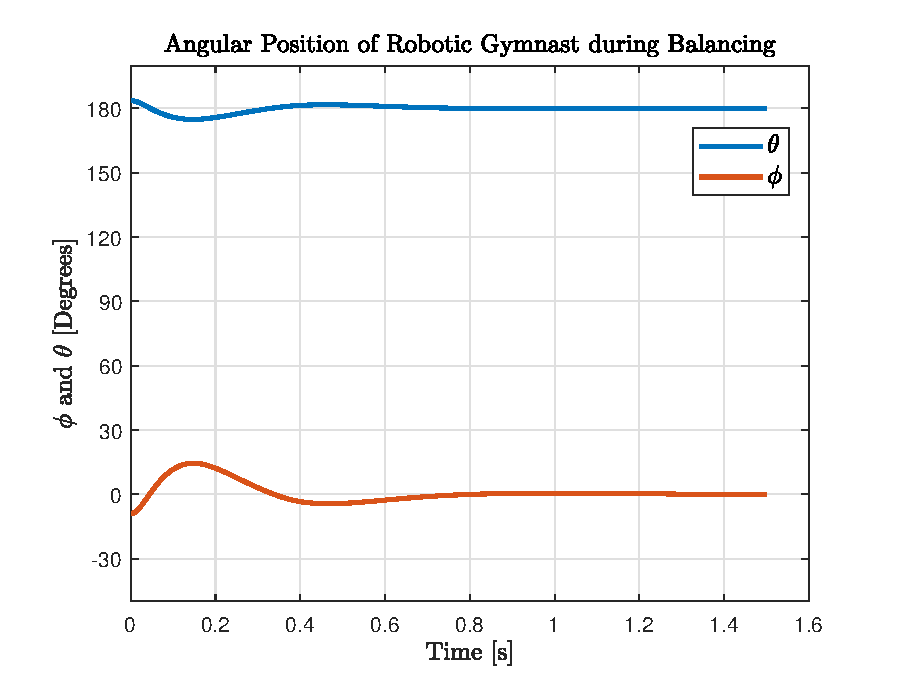
\includegraphics[scale=1]{./figs/balancing}
	\caption{Balancing of the Robotic Gymnast}
	\label{fig:balance}
\end{figure}



Figure \ref{fig:balance} shows the robotic gymnast balancing around the unstable equilibrium position from an initial condition of $$ \vec{q} = 
\begin{bmatrix}
\pi + \frac{\pi}{50}\\
-\frac{\pi}{25}
\end{bmatrix}
$$ 

The response shows that the controller meets the requirement of balancing the robotic gymnast from initial condition of $q \in []$ and reaches steady state within 1 seconds. The overshoot requirement of 10\% has also been achieved on the unactuated pendulum.\\

The identified coulomb damping that the unactuated pendulum experience is not possible to linearised (ref). This friction was approximated as viscous damping in the linear model and was acceptable due to the physical model showing characteristic of viscous damping near steady state visible in Figure \ref{fig:q1_response}.



\section{Swingup Controller}
% WHAT you are going to present in this chapter/section
% WHY you are presenting it, and
% HOW you are going to present it
For the robotic gymnast to swing from the stable equilibrium position to the unstable equilibrium position the feedback control must incorporate the non-linearities of the system. How these non-linearities of the system are incorporated and the design approach to swinging will be explained in the following section.

\subsection{Controller Architecture}
\begin{figure}[h]
	\centering
	\documentclass{article}

\usepackage{tikz}
\usetikzlibrary{shapes,arrows}
\usepackage{amsmath,bm,times}
\newcommand{\mx}[1]{\mathbf{\bm{#1}}} % Matrix command
\newcommand{\vc}[1]{\mathbf{\bm{#1}}} % Vector command

\begin{document}
	\pagestyle{empty}
	
	% We need layers to draw the block diagram
	\pgfdeclarelayer{background}
	\pgfdeclarelayer{foreground}
	\pgfsetlayers{background,main,foreground}
	
	% Define a few styles and constants
	\tikzstyle{sensor}=[draw, fill=blue!20, text width=5em, 
	text centered, minimum height=2em]
	\tikzstyle{ann} = [above, text width=5em]
	\tikzstyle{block} = [sensor, text width=6em, fill=red!20, 
	minimum height=4em, rounded corners]
	\tikzstyle{sum}=[draw, fill=red!20, circle, node distance = 2cm]
	
	\tikzstyle{longblock} = [sensor, text width=10em, fill=red!20, 
	minimum height=4em, rounded corners,minimum width=6em]
	
	\def\blockdist{2.5}
	\def\edgedist{2.5}
	
	
	
	\noindent\makebox[\textwidth]{
	\begin{tikzpicture}[scale=0.8]
	% plant block
	\node (plant) [block] {Non-Linear Plant};
	
	% collocated blovk
	\path (plant)+(0,-\blockdist) node (collinear) [block] {Collocated\ Linearisation};
	
	% Annotation
%	\path (plant)+(1.5*\blockdist,0) node (output) [ann] { [ $\ddot{\theta}$ \\ $\dot{\phi}$ ] };
	
	\path (plant)+(1.2*\blockdist,0) node (output) [ann] { 
$\begin{bmatrix}
$$\ddot{\theta}$$ \\ $$\ddot{\phi}$$ 
\end{bmatrix}$
};
	
	%sumation block 1
	\path (plant)+(-\blockdist,0) node (suma1) [sum]{\Large$\Sigma$};
	
	% Non-linear control law
	\path (plant)+(-2.2*\blockdist,0) node (nonlinear) [longblock]{Non-Linear Law \ $v = K_{p}(\phi^{d}-\phi)-K_{d}\dot{\phi}$};
	
	%sumation block 2
	\path (nonlinear)+(-1.2*\blockdist,0) node (suma2) [sum]{\Large$\Sigma$};

	% Desired input
	\path (suma2)+(-1.2*\blockdist,0) node (desired) [longblock]{Desired Trajectory \ $\phi^{d} = \alpha \tan(\dot{\theta})$};

%%%%%%%%%%%%%%%%%%%%%%%%%%%%%%%%%%%%%%%%%%%%%%%%%%%%%%%%%%%%%%%%%%%%%%%%%%%%%%%%%%%%%%%%%%%%%%%%%%%%%%%%%%%%%%%%%%%%%%%%%%
	% plant to output	
%	\draw [->,thick] (plant) -- node [anchor=north east] {} + (\edgedist,0) 
%	node[right] {$[\theta$ $\phi$ $\dot{\theta}$ $\dot{\phi}$ $\ddot{\phi}$  $\ddot{\theta}]$};
	
	%plant to output
	\draw [->,thick] (plant.east) -- ([xshift=1cm]plant.east) {};
	% plant to collocated
	\draw[->,thick] ([xshift=0.5cm]plant.east) -- ([xshift=0.5cm]collinear.east) -- (collinear.east) {};
	
	% collocated lineariation to Sigma
	\draw[->,thick] (collinear.west) -| (suma1.south) {};
	
	%sigma to non-linear plant
	\draw[->,thick] (suma1.east) -- (plant.west) {};
	
	% non-linear law to sigma
	\draw[->,thick] (nonlinear.east) -- (suma1.west) {};
	
	% sigma2 to non linear
	\draw[->,thick] (suma2.east) -- (nonlinear.west) {};

	% Desired input to sigma
	\draw[->,thick] (desired.east) -- (suma2.west) {};
	
	% collocated to sigm2
	\draw[->,thick] (collinear.west) -| (suma2.south) {};
	






	% Now it's time to draw the colored IMU and INS rectangles.
	% To draw them behind the blocks we use pgf layers. This way we  
	% can use the above block coordinates to place the backgrounds   
	\begin{pgfonlayer}{background}
	% Compute a few helper coordinates
%	\path (gyros.west |- naveq.north)+(-0.5,0.3) node (a) {};
%	\path (INS.south -| naveq.east)+(+0.3,-0.2) node (b) {};
	%\path[fill=yellow!20,rounded corners, draw=black!50, dashed]
	%(a) rectangle (b);
%	\path (gyros.north west)+(-0.2,0.2) node (a) {};
	%\path (IMU.south -| gyros.east)+(+0.2,-0.2) node (b) {};
%	\path[fill=blue!10,rounded corners, draw=black!50, dashed]
%	(a) rectangle (b);
	\end{pgfonlayer}

\end{tikzpicture}
}
	
\end{document}
	\caption{Block Diagram of the Non-Linear Controller}
	\label{fig:nonlinear_controller_arch}
\end{figure}

Figure \ref{fig:nonlinear_controller_arch} shows a high-level block diagram of the multiple parts of the swing-up controller. These parts are required to work in unison to allow the robotic gymnast to swing.\\

The collocated linearisation block is the foundation on which the entire controller was built. It creates a linear response from one of the outputs of the plant. This linear response can then be used to follow a desired trajectory.\\

The swing-up controller implements classical control theory approach where gains are selected to characterise the response of the system based on the error of the desired trajectory and the actual trajectory of the system.\\

Each of the blocks shown in the block diagram will be discussed in the section below.


\subsection{Requirements/Specifications and Constraints}
% WHAT you are going to present in this chapter/section
% WHY you are presenting it, and
% HOW you are going to present it
The requirements of the swing-up controller is to swing the robotic gymnast upwards under 30 seconds in the vicinity of the unstable equilibrium position. The vicinity of the unstable equilibrium position is defined as $\theta = \SI{2\pi}{\radian} \pm \frac{\pi}{30}$ and $\phi \in [-5^{\circ},5^{\circ}]$.\\

Constraints that are placed on the controller are not to use 50\% of the stall torque of the motor during the entire swing-up of the robotic gymnast.\\

The first requirement is to provide a feasible solution to the swing-up of the robotic gymnast and allow the swing-up sequence to be captivating. The second requirement is to ensure the linear approximation of the system is acceptable when the balancing controller is active to bring the system to the inverted position and balance. The constraint placed was to increase the safety in testing and prolonging the life of the motor.\\

\subsection{Feedback Linearisation}
It has been shown that it is not possible to linearise the dynamics of the gymnast by means of static state feedback and non-linear transformation \citep{murray}, but it is possible to achieve a linear response from one of the outputs of the plant by implementing a non-linear feedback. This non-linear feedback is the partial feedback linearisation.\\

Collocated linearisation is a form of partial feedback linearisation where a non-linear control input $\tau$ is used to linearise the response of the actuated pendulum $\ddot{\phi}$. By analysing equation (\ref{eq:condense2}), the input $\tau$ was chosen to cancel all the non-linearities of the system and add an additional outer loop control input $v_{2}$ as seen in equation (\ref{eq:collocated_lin3}). This results in the unactuated pendulum to see a indirect force and the problem can be reduced to finding the outer loop control input to force the actuated pendulum to swing upwards \citep{spong_swingup}.

 The derivation of the collocated linearisation is shown in Appendix \ref{sec:colocated_linearisation}.
\begin{equation} \label{eq:collocated_lin3}
\tau = d_{21}\ddot{\theta} + v_{2}d_{22}\ddot{\phi} + h_{2} + \psi_{2}
\end{equation}
\begin{equation} \label{eq:collocated_lin1}
d_{11}\ddot{\theta} + h_{1} + \psi_{1} = -d_{12}v_{2} \approx F
\end{equation}
\begin{equation} \label{eq:collocated_lin2}
\ddot{\phi} = v_{2}
\end{equation}

The subtle practical implication of using collocated linearisation is that the system being controlled must be well defined. If this is not the case the non-linear input $\tau$ will introduce other unwanted dynamics that could lead to undesirable behaviour.

\subsection{Nonlinear Control Law}

The ability to control the actuated pendulum to follow a desired trajectory, provides the possibility to increase the energy of the system if the correct trajectory is chosen. The increase of energy in the system will cause the pendulums to rise from their stable equilibrium position and start swinging upwards. The desired trajectory for ${\phi}$ was chosen as equation (\ref{eq:desired_phi}) determined by \citet{spong_swingup}.
\begin{equation} \label{eq:desired_phi}
\phi^{d} =  \alpha \arctan(\dot{\theta})
\end{equation}

This desired trajectory was derived by analysing a single pendulum and approximating the force it experiences as seen in equation (\ref{eq:collocated_lin1}). By using this approximation \citet{spong_swingup} shows that the desired trajectory will increase the energy in the system. The desired trajectory also tries to allow the actuated pendulum to swing in phase with the non-actuated pendulum and by this approach the energy of the actuated pendulum is transferred to the unactuated pendulum \citep{spong_swingup}.\\

The outer loop control input, $v_{2}$, then implements the classical control approach where gains are selected to characterise the response of the system based on the error seen in equation (\ref{eq:v2}). 

   
\begin{equation} \label{eq:v2}
v_{2} = K_{p}(\phi^{d}-\phi)-K_{d}\dot{\phi}
\end{equation}

The coefficient $\alpha$ used in equation (\ref{eq:desired_phi}) constrains the actuated pendulum to stay within a interval of $ \phi \in [-\beta,\beta]$ where $\alpha < \beta$ \citep{spong_swingup}. This provides better control over the system to stay within the null controllability region when the system reaches the unstable equilibrium position.\\

Another side-effect of using the non-linear controller is that at rest the system will not start to swing-up. At rest, the conditions are: $\phi = \SI{0}{\radian}$ and $\dot{\phi} = \SI{0}{\radian/s}$, and results in the control output seen in equation (\ref{eq:v2}) to be zero. This effect was overcome by giving the system a small initial condition to start the swing-up controller.


\subsection{Simulation Response}
\begin{figure}[h]
	\centering
	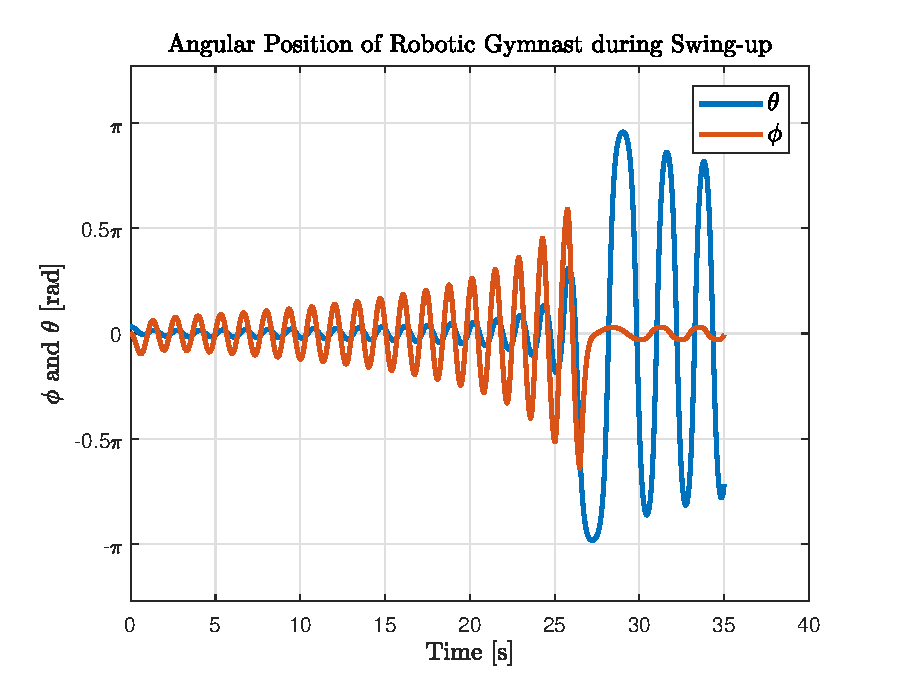
\includegraphics[scale=1]{./figs/swingup}
	\caption{Swing-up of the Robotic Gymnast}
	\label{fig:swingup}
\end{figure}

Figure \ref{fig:swingup} shows the swing-up controller swinging the robotic gymnast from the stable equilibrium position to the vicinity of the unstable equilibrium position with gain constants used shown in Table \ref{table:gain_constants}. There are a few interesting occurences in the responses mentioned in the previous section which needs to be brought to the attention of the reader.\\

\begin{table}[]
	\centering
	\begin{tabular}{|c|c|}
		\hline
		Gain Constant & Value \\
		\hline
		\hline
		$K_{p}$  & 58 \\
		\hline
		$K_{d}$  & 14 \\
		\hline
	\end{tabular}
	\caption{}
	\label{table:gain_constants}
	\end{table}

Firstly the robotic gymnast is required to start at an initial condition for the swing-up control law to be active and this is seen with $\theta$ starting at 11\textdegree. Secondly, the amplitude of $\phi$ is seen to decrease suddenly when the system nears the inverted position. This is due to $\alpha$ being reduced when the robotic gymnast nears the inverted position.\\

The response shows the swing-up controller meets the designed requirements by swinging the robotic gymnast to the vicinity of the unstable equilibrium within 30 seconds and $\theta$ and $\phi$ are in the designed region for the balancing controller to bring the system to the inverted position.



\section{Simulation Results}
\begin{figure}[h]
	\centering
	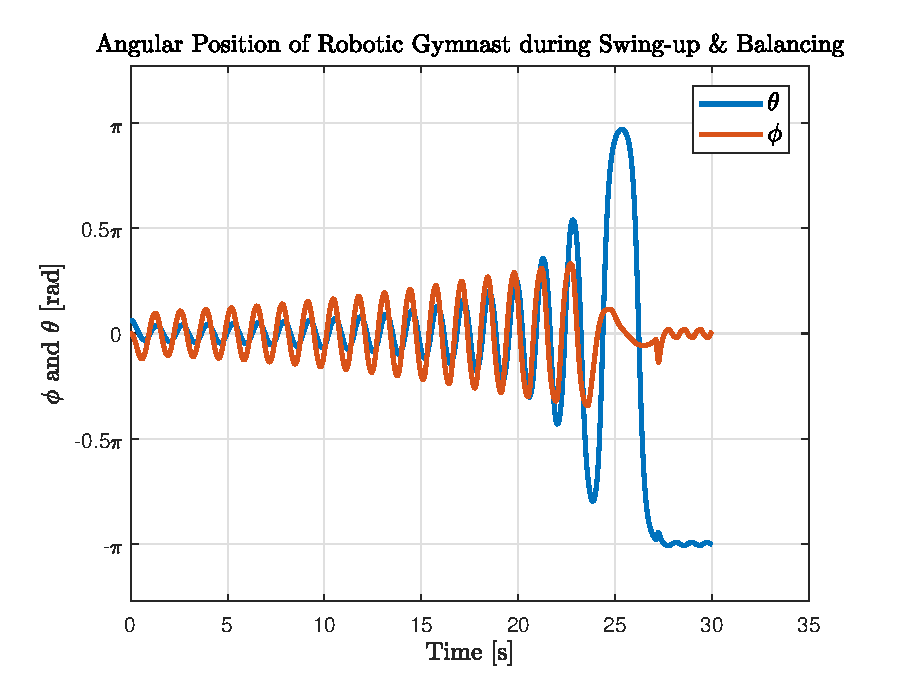
\includegraphics[scale=1]{./figs/swingup_balance}
	\caption{The Swing-Up \& Balancing of the Robotic Gymnast}
	\label{fig:swingup_balance}
\end{figure}

Once both controllers were capable of meeting the requirements set out, they needed to be combined to achieve the swing-up and balancing of the robotic gymnast. Figure \ref{fig:swingup_balance} shows the response of both controllers combined that achieved the swing-up and balancing.\\

During the swing-up the $\alpha$ value was reduced as the robotic gymnast started nearing the unstable equilibrium position as seen below.


$$ \alpha = 
\left \{
\begin{tabular}{cc}
$ \frac{\pi}{2} $ & $  \frac{-\pi}{2} < \theta < \frac{\pi}{2} $\\
$ \frac{\pi}{12} $ & $ $\\
$ \frac{\pi}{24}  $ &   $  \frac{-\pi}{1.1} >\theta \theta > \frac{\pi}{1.1}$ \\
\end{tabular}
\right \}
$$

